
\section{processes.xml}

The process file is used to define constraints related to complex
cellular processes.

\subsection{RBAProcesses}
\label{sec:rba_processes}

The outermost portion of the process file is an instance of class
\rbaprocesses, shown in Figure~\ref{fig:processes_doc}.

\begin{figure}
  \centering
  \includegraphics[scale=0.9]{figures/processes_doc}
  \caption{XML structure of process document.}
\label{fig:processes_doc}
\end{figure}

\rbamacromolecules{} has no simple attributes.
It contains exactly one instance of \textbf{ListOfProcesses}
and \textbf{ListOfComponentMaps}.


\subsection{Process}
\label{sec:process}

The \process{} class is used to define cellular processes
(Fig.~\ref{fig:processes_process}).
Processes cover a wide variety of non-metabolic reactions.
We encourage you to study existing example to understand how the different
substructures are used.

\begin{figure}
  \centering
  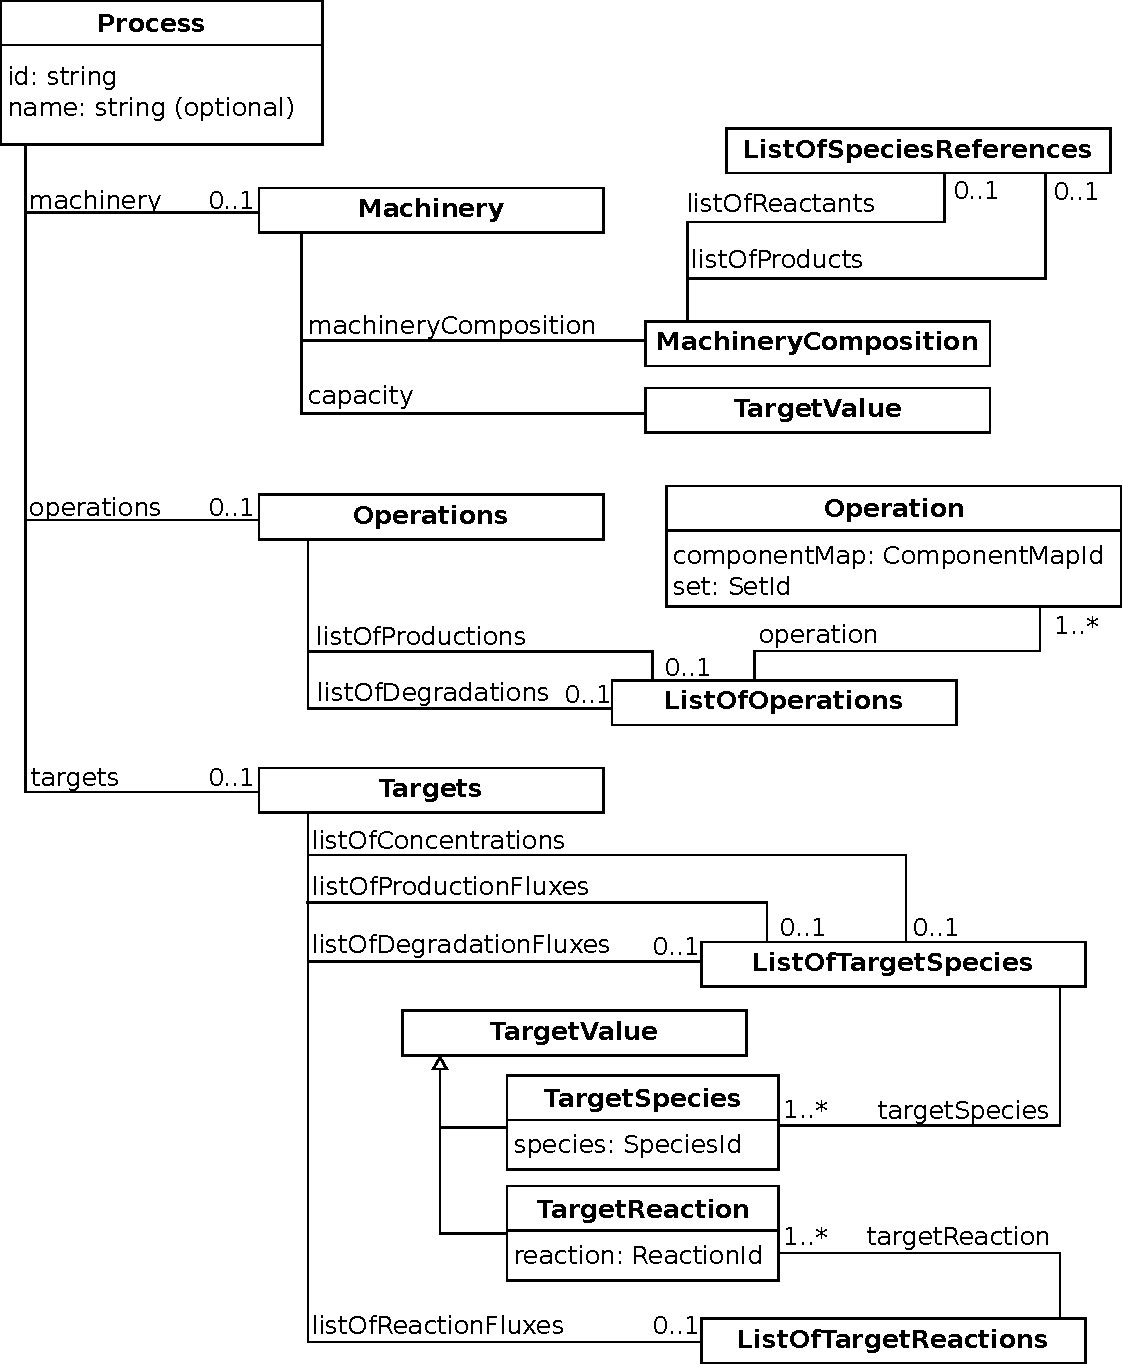
\includegraphics[scale=0.9]{figures/processes_process}
  \caption{Class used to store processes.}
\label{fig:processes_process}
\end{figure}

\paragraph{The \textit{id} attribute}
The \textbf{id} attribute is a string defining the identifier of a process.


\subsection{ComponentMap}
\label{sec:component_map}

The \componentmap{} class is used to define how \process{}es assemble or
disassemble \macromolecule{}s (Fig.\ref{fig:processes_component_map}).

\begin{figure}
  \centering
  \includegraphics[scale=0.9]{figures/processes_component_map}
  \caption{Class used to store production/degradation of macromolecules.}
\label{fig:processes_component_map}
\end{figure}

\paragraph{The \textit{id} attribute}
The \textbf{id} attribute is a string defining the identifier of a
component map.
